\documentclass[12pt]{article}

\usepackage[affil-it]{authblk}
\usepackage[shortlabels]{enumitem}
\usepackage[utf8]{inputenc}
\usepackage{algorithm, algorithmicx, algpseudocode}
\usepackage{amsfonts, amsthm, amsmath, amssymb}
\usepackage{color}
\usepackage{cancel, textcomp}
\usepackage{enumerate}
\usepackage[mathscr]{euscript}
\usepackage{fancyhdr, fancyvrb}
\usepackage{fullpage}
\usepackage[left=0.5in,right=0.5in,headsep=0.5in,headheight=0.5in]{geometry}
\usepackage{graphicx}
\usepackage{hyperref}
\usepackage{latexsym}
\usepackage{mathtools}
\usepackage{minted}
\usepackage{times}
\usepackage{xcolor}
\usepackage{physics}
\usepackage{tikz-cd}
\usepackage[warnunknown, fasterrors, mathletters]{ucs}
\usepackage[nointegrals]{wasysym}

\newcommand{\hw}[2]{
    \noindent
    \begin{center}
        \framebox{
            \vbox{
                \hbox to 7in { {\bf MATH 470: Communications and Cryptography } \hfill  }
                \vspace{2mm}
                \hbox to 7in { {\Large \hfill Homework #1\hfill} }
                \vspace{2mm}
                \hbox to 7in { {\it Due date: #2 \hfill Name: Huy Lai } }
            }
        }
    \end{center}
    \vspace*{4mm}
}

\newcounter{prob}
\setcounter{prob}{0}
\newcounter{subprob}
\setcounter{subprob}{0}

\newcommand{\problem}{\setcounter{subprob}{0}\stepcounter{prob}{\noindent\textbf{Problem \theprob.}}\ }
\newcommand{\subproblem}{\stepcounter{subprob}{\noindent\textbf{Subproblem \thesubprob.}}\ }
\newcommand{\solution}{\noindent\textbf{Solution:}\newline}

\newcommand{\babc}{\begin{enumerate}[a)]}
\newcommand{\eabc}{\end{enumerate}}

\everymath{\displaystyle}

\setlength{\parskip}{.1in}
\setlength{\headheight}{15pt}
\setlength{\topmargin}{0pt}

\fancyhf{}
\pagestyle{fancy}
\lhead{MATH 470: Communications and Cryptography}
\rhead{Texas A\&M University}
\cfoot{\thepage}


\begin{document}
\thispagestyle{empty}
\hw{9}{15 November 2023}

\problem Solve the discrete logarithm problem $10^x=106$ in the finite field $\mathbb{F}_{811}$ by finding a collision among the random powers $10^i$ and $106\cdot10^i$ that are listed in Table 5.17.

\solution
From the table we see that
\[10^{234}=106\cdot10^{399}=304\quad\text{in}\quad\mathbb{F}_{811}\]
Hence
\[10^{234}\cdot10^{-399}=10^{-165}=10^{645}=106\quad\text{in}\quad\mathbb{F}_{811}\]

\newpage
\problem Program Pollard's $\rho$ algorithm with $f(x)=x^2+1$ and $x_0=y_0=0$, and use it to factor the following numbers. In each case, give the smallest value of $k$ such that $g_k$ is a non trivial factor of $N$ and print the ratio $\frac{k}{\sqrt{N}}$
\begin{enumerate}
    \item $N=2201$
    \item $N=9409613$
    \item $N=1782886219$
\end{enumerate}

\solution
\inputminted{py}{pollard.py}

\begin{figure}[!ht]
    \centering
    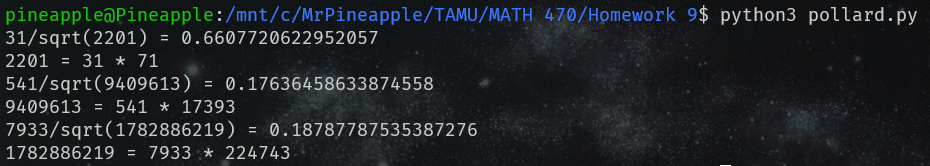
\includegraphics[width=\textwidth]{Question 2.png}
    \caption{Output}
\end{figure}

\newpage
\noindent
For Question 3 through 6 consider the following protocol (Schnorr Signature):

\noindent
Let $p$ be a large prime of the form $p=2q+1$ where $q$ is prime.\\
Let $g\in(\mathbb{Z}/p\mathbb{Z})^*$ be an element of order $q$.\\
Let $\langle g\rangle$ denote the set $\{1,g,g^2,g^2,\cdots,g^{q-1}\mod{p}\}$. (note that $g$ is not a primitive root $\mod{p}$, and $\langle g\rangle$ only contains half the numbers in $(\mathbb{Z}/p\mathbb{Z})^*$)\\
Assume that discrete logarithm problem for $p,g$ is hard. In other words, assume that there is no efficient algorithm that can compute, for any given $A\in\langle g\rangle$, an integer $a$ such that $g^a\equiv A\mod{p}$.\\
Let $A\in\langle g\rangle$.\\
Peggy wants to convince Victor that she knows an integer $a$ such that $g^a\equiv A\mod{p}$.
\begin{itemize}
    \item Peggy chooses a random integer $c\in\mathbb{Z}/q\mathbb{Z}$, computes $C=g^c\mod{p}$, and sends \textbf{commitment} $C$.
    \item Victor chooses a random integer $h\in\mathbb{Z}/q\mathbb{Z}$, and sends \textbf{challenge} $h$.
    \item Peggy computes $r=c+ah\mod{q}$, and sends \textbf{response} $r$.
    \item Victor \textbf{accepts} if $g^r\equiv C\cdot A^h\mod{p}$, and \textbf{rejects} otherwise.
\end{itemize}

\newpage
\problem Let $x$ be an integer with $x\not\equiv0\mod{q}$. Prove that there exists an integer $y$ such that $g^{xy}\equiv g\mod{p}$

\solution
The proof is as follows
\begin{proof}
    Since $g$ has order $q$, we get that
    \[g^q\equiv 1\mod{p}\]

    \noindent
    We can rewrite $g^{xy}\equiv g\mod{p}$ as
    \[g^{xy-1}\equiv 1\mod{p}\]

    \noindent
    Since $q$ is the order, by proposition we know that $q\mid(xy-1)\rightarrow\exists k\in\mathbb{Z},xy=kq+1$.\\
    We can plug this into the original equation we get
    \begin{flalign*}
        g^{xy-1}     & \equiv 1\mod{p} & \\
        g^{(kq+1)-1} & \equiv 1\mod{p} & \\
        (g^q)^k      & \equiv 1\mod{p} & \\
        1^k          & \equiv 1\mod{p}
    \end{flalign*}
    Therefore we can find a $y$ such that $g^{xy}\equiv g\mod{p}$.\\
    This $y$ can be found by solving the congruence $xy\equiv 1\mod{q}$
\end{proof}

\problem Prove that the above protocol satisfies \textbf{completeness}; that is, prove that if Peggy does know $a$ and if both parties follow the protocol, then Victor always accepts.

\solution
We can verify that $g^r$ is sufficient enough for Victor to verify as follows
\begin{flalign*}
    g^r & \equiv g^{c+ah}                & \\
        & \equiv g^c\cdot (g^a)^h\mod{p} & \\
        & \equiv C\cdot A^h\mod{p}
\end{flalign*}
Since the discrete log problem is assumed hard for $g,p$, Victor can have confidence that Peggy did not calculate $a$ and instead knows $a$.

\newpage
\problem A transcript is a tuple $(C,h,r)$ where $C\in\langle g\rangle,h\in\mathbb{Z}/q\mathbb{Z}$. A transcript $(C,h,r)$ is valid if $g^r\equiv C\cdot A^h\mod{p}$.
Prove that if you are given two valid transcripts $(C,h_1,r_1)$ and $(C,h_2,r_2)$ with $h_1\not\equiv h_2\mod{q}$, then you can efficiently compute $a$. (This property is called special \textbf{soundness}).

\solution
From the valid certificates we can generate the following system of congruence
\begin{align*}
    g^{r_1} & \equiv C\cdot A^{h_1}\mod{p} \\
    g^{r_2} & \equiv C\cdot A^{h_2}\mod{p}
\end{align*}
Dividing these two equivalences gives
\begin{align*}
    g^{r_1-r_2} & \equiv A^{h_1-h_2}\mod{p}     \\
                & \equiv (g^a)^{h_1-h_2}\mod{p} \\
    r_1-r_2     & =a(h_1-h_2)
\end{align*}
Solving this equation gives
\[a=\frac{r_1-r_2}{h_1-h_2}\]

\newpage
\problem Prove that the above protocol satisfies honest verifier zero knowledge; that is, prove that there is an efficient algorithm which, without knowledge of $a$, can produce transcripts that are indistinguishable from transcripts of honest interactions between Peggy (who knows $a$) and Victor.

\solution
To generate transcripts that are indistinguishable from honest interactions between Peggy and Victor, we need to generate tuples $(C,h,r)$ that are distributed identity to those send between Peggy and Victor.

\noindent
We can generate this transcript by running the protocol algorithm in reverse.
\begin{enumerate}
    \item Let $r\in\mathbb{Z}/q\mathbb{Z}$ be a uniformly random integer.
    \item Let $h\in\mathbb{Z}/q\mathbb{Z}$ be a uniformly random integer.
    \item Let $C\equiv g^r\cdot A^{-h}\mod{p}$
\end{enumerate}
We can verify the following this process, a verify could compute the following
\begin{flalign*}
    g^r & \equiv C\cdot A^{h}\mod{p}             & \\
        & \equiv g^r\cdot A^{-h}\cdot A^h\mod{p} & \\
        & \equiv g^r
\end{flalign*}
This means that with an exchange constructed with this method, a reader of a transcript $(C,h,r)$ can be independently verified as accepted relations.
However, this does not prove to the transcript reader that Peggy actually knows the secret.
\end{document}